\documentclass[preprint,12pt]{elsarticle}
\usepackage{fontspec}
\defaultfontfeatures{Ligatures=TeX}
\setmainfont{Times New Roman}
\setsansfont{Times New Roman}
\setmonofont{Courier New}
\usepackage{amsmath,mathtools,unicode-math}
\setmathfont{STIX Two Math}
\usepackage{graphicx,booktabs,tabularx,xltabular,array,ragged2e}
\usepackage{caption,float,placeins,needspace}
\usepackage{lineno,setspace,microtype}
\usepackage{enumitem,xcolor}
\usepackage{algorithm}
\usepackage{algpseudocode}
\usepackage[hidelinks]{hyperref}
\hypersetup{pdftitle={Scale-Explicit and Uncertainty-Qualified Assessment of Tangent-Only Matrix Perturbations in Coupled Finite-Element Linearizations}}
\renewcommand{\tabularxcolumn}[1]{>{\RaggedRight\arraybackslash}p{#1}}
\renewcommand{\arraystretch}{1.14}
\captionsetup{font=small,labelfont=bf,skip=5pt}
\setlength{\parindent}{1.5em}
\setlength{\parskip}{0.08em}
\setlength{\emergencystretch}{2em}
\setstretch{1.04}
\journal{Computer Methods in Applied Mechanics and Engineering}

\begin{document}
\begin{frontmatter}

\title{Scale-Explicit and Uncertainty-Qualified Assessment of Tangent-Only Matrix Perturbations in Coupled Finite-Element Linearizations}
\author[aff1]{Bing Liang}
\author[aff1]{Yangqi Ma}
\author[aff1]{Weiji Sun\corref{cor1}}
\ead{sunweiji-1231@163.com}
\author[aff2]{Shi He}
\cortext[cor1]{Corresponding author.}
\address[aff1]{School of Mechanics and Engineering, Liaoning Technical University, No. 47 Zhonghua Road, Fuxin, Liaoning 123000, China}
\address[aff2]{China Coal Research Institute, Beijing 100013, China}

\begin{abstract}
Tangent-only matrix perturbations are often judged by their norm relative to a finite-element tangent, although the realized directional response also depends on inverse amplification, probe direction, coordinate representation, and finite-precision resolvability. Existing perturbation, scaling, and floating-point tools do not by themselves provide a coordinate-explicit procedure for qualifying the response of a selected coupled linearization. We develop a scale-explicit and uncertainty-qualified assessment that declares the solved space and coordinates, separates matrix, operator, and realized directional measures, and evaluates each arithmetic route against its own error enclosure. Its mathematical basis combines an exact finite response identity, consistent transformation of the operator and perturbation, and a zero-exclusion criterion under route-specific uncertainty. Pre-specified synthetic families verified a six-amplitude directional counterexample, coordinate transformation and redeclaration, and complete development/holdout uncertainty coverage under decimal-source and binary64-operand truth contracts. The procedure was then applied separately to two independently frozen coupled finite-element linearizations of dimensions 196 and 900. Direct-difference and response-equation routes excluded zero in both applications under their respective route-specific uncertainties. These results show that matrix-space smallness alone does not determine a realized response and that numerical distinguishability requires explicit coordinate and arithmetic-route declarations. The two applications demonstrate replication of the procedure, not guard safety, nonlinear prediction, or generality across finite-element systems.
\end{abstract}

\begin{keyword}
tangent matrix \sep matrix perturbation \sep finite-element linearization \sep coordinate scaling \sep floating-point uncertainty \sep directional response
\end{keyword}

\end{frontmatter}
\linenumbers

\section{Introduction}

Coupled nonlinear finite-element analyses repeatedly form local or global tangent systems whose blocks represent variables with different units and characteristic scales. Implementations may add a small diagonal or structured matrix term to avoid singular factorization, regularize an intermediate solve, or continue an iteration through a difficult local linearization. We call such a change a \emph{tangent-only matrix perturbation} when it modifies the matrix supplied to the linear solve without adding the corresponding term to the residual. This object is narrower than residual-consistent finite-element stabilization and should not inherit claims about consistency, mixed-method stability, conservation, or boundedness. Field-aware solvers and matrix normalization are active computational choices in coupled finite-element systems \cite{S17,S20,S29,S30}; the response induced by a tangent-only change therefore requires a separate assessment.

A matrix perturbation is commonly described as small when $\lVert\Delta J\rVert/\lVert J\rVert$ is small. That ratio answers how much the declared matrix changed in one norm and coordinate system, but not how one selected right-hand side responds. The realized change also depends on inverse propagation and on the direction of $\Delta Jz$. Equal matrix-space amplitudes can consequently produce different solution responses, while a condition number supplies a worst-case sensitivity comparison rather than a directional explanation \cite{S01,S02,S03}. This distinction matters in mixed-field mechanics because the same numeric diagonal coefficient can act beside displacement, pressure, or internal-variable blocks whose coordinates and residual scales differ by many orders of magnitude.

Matrix perturbation theory provides exact response identities and norm bounds; conditioning theory separates forward sensitivity from backward error; scaling and equilibration expose coordinate dependence; and floating-point analysis explains why subtracting two accurate parent solutions may not resolve their small difference \cite{S02,S03,S05,S06,S08,S09,S10,S11}. Verified computing and precision-aware refinement offer routes for constructing reference enclosures \cite{S12,S13,S28}. These bodies of theory are essential, but they do not by themselves form a coordinate-explicit, probe-aware, route-specific procedure for qualifying the numerical response induced by a tangent-only perturbation in a selected coupled finite-element linearization.

The computational gap is therefore one of integration and declaration. An interpretable assessment must fix the solved space, unknown and residual coordinates, norm, right-hand side, perturbation operator, arithmetic response route, and numerical truth object before comparing values. It must then keep matrix amplitude, inverse-mediated amplification, and realized response distinct, and it must qualify the observed response with an error enclosure matched to the operations that produced it. Without these declarations, a small coefficient, a small backward error, or a high-precision difference can each answer a different question while appearing to support the same conclusion.

We propose a scale-explicit and uncertainty-qualified computational assessment procedure for this purpose. The procedure consistently transforms $J$, $\Delta J$, and $b$; evaluates matrix, operator, and directional quantities in declared coordinates; applies the exact finite response relation; builds an uncertainty budget for the selected arithmetic route; and classifies only whether the resulting response interval excludes zero. Figure~\ref{fig:1} gives the conceptual sequence, and Algorithm~\ref{alg:assessment} supplies its executable presentation. The procedure does not select a perturbation or define a universal acceptance threshold.

The contribution has four parts. First, an exact two-dimensional construction proves that matched matrix amplitude, condition number, and finite worst-direction amplification do not determine a realized directional response. Second, a coordinate analysis distinguishes transformation of one fixed perturbation from redeclaration of a same-numeric identity after rescaling. Third, a two-contract uncertainty model separates decimal-source and binary64-operand truth objects and qualifies direct-difference and response-equation routes independently. Fourth, the complete procedure is validated on pre-specified synthetic families and applied independently to two frozen coupled finite-element tangent systems.

The validation hierarchy is deliberately layered. Analytical constructions verify the directional and coordinate statements. Development and disjoint holdout families test uncertainty coverage within specified operator classes and dimensions. The two finite-element applications then use immutable 196- and 900-dimensional binary64 operand snapshots, independent high-precision references, and route-specific error enclosures. These applications demonstrate replication on two coupled linearizations; they are not a mesh sequence or a statistical sample of finite-element systems.

\begin{figure}[htbp]
\centering
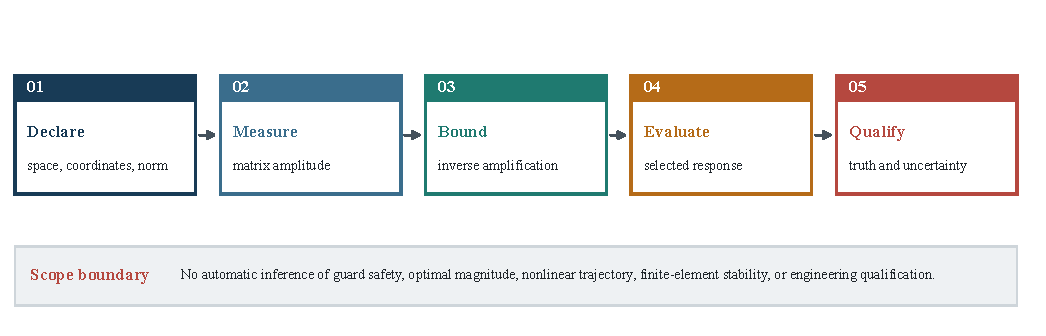
\includegraphics[width=0.90\linewidth,height=0.62\textheight,keepaspectratio]{F1_assessment_sequence.pdf}
\caption{Computational sequence from solved-space and coordinate declaration to route-specific uncertainty-qualified response interpretation.}
\label{fig:1}
\end{figure}

Section~2 defines the mathematical and computational framework. Sections~3--5 verify the directional construction, coordinate transformation, and uncertainty model. Section~6 applies the procedure to the two coupled finite-element linearizations, and Section~7 discusses interpretation, scalability, and limitations.

\FloatBarrier
\section{Mathematical and Computational Framework}

\subsection{Problem definition and solved-space contract}

Consider an unguarded linear system and a matrix-perturbed system posed on the same solved space. The matrices $J$ and $J + \Delta J$ are assumed square and nonsingular, both systems use the same right-hand side $b$, and their solutions are represented in one fixed coordinate system. A constrained problem may enter this framework only after its free or otherwise reduced solved space has been declared; no assertion is made for an unreduced singular operator. We write $\lVert . \rVert$ for one declared vector norm and its associated subordinate matrix norm, so all matrix-vector and matrix-matrix product bounds use the same convention. The comparison therefore concerns two operators acting on the same data, not two problems with different loads, coordinates, nullspaces, or residual roots. These requirements are the minimum conditions under which a finite solution-response identity and its norm bounds have a single interpretation \cite{S02,S03}.

\subsection{Matrix, operator, and directional measures}

The unguarded solution is denoted by $z$, the guarded solution by $z_g$, and their difference by $\delta z = z_g - z$. Six quantities are retained because they answer different questions. The matrix ratio $\mu_J$ measures perturbation amplitude in the declared coordinates; $\rho_1$ measures first-order worst-direction amplification through the unguarded inverse; $\rho_g$ measures finite guarded-inverse amplification; $\eta_z$ measures the realized relative response for the selected right-hand side; $G_g$ reports the diagnostic ratio between that realized response and matrix amplitude when $\mu_J$ is nonzero; and $\kappa(J)$ measures normwise sensitivity of the unguarded linear problem. None of these quantities substitutes for another. In particular, an operator norm is not the response of a selected probe, and a condition number is not a causal classification of an observed change \cite{S01,S03}. Taken together, the quantities define an assessment chain rather than a composite guard-quality score.

Figure~\ref{fig:2} places a tangent-only perturbation within a generic mixed-field block operator without assigning physical meaning to one scalar diagonal coefficient.

\begin{figure}[htbp]
\centering
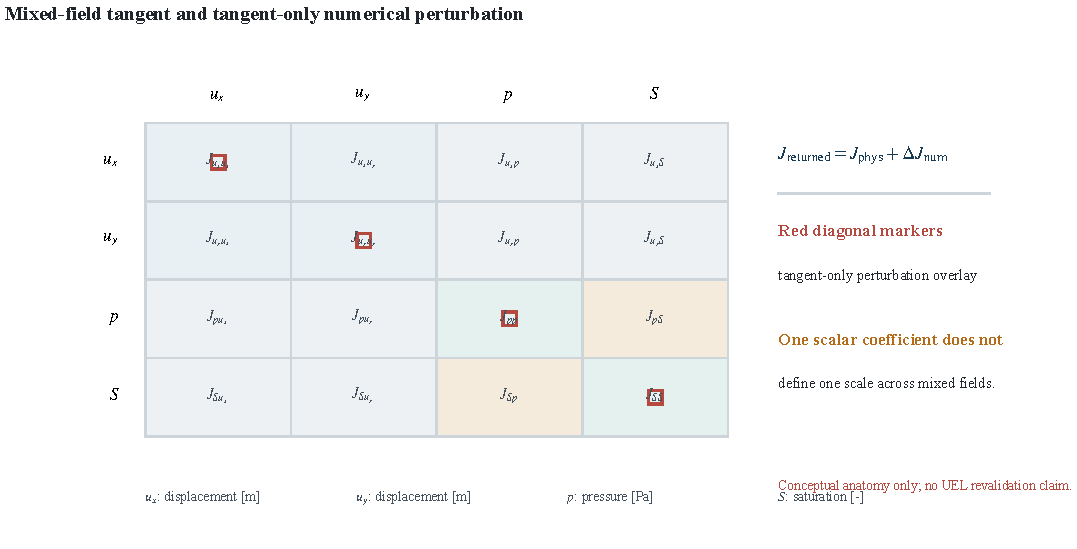
\includegraphics[width=0.90\linewidth,height=0.62\textheight,keepaspectratio]{F2_mixed_field_tangent_anatomy.pdf}
\caption{Generic mixed-field tangent with a tangent-only diagonal perturbation shown as a separate matrix overlay.}
\label{fig:2}
\end{figure}

Table~\ref{tab:1} lists the retained metrics and their non-substitution rules.

\begin{table}[htbp]
\centering
\small
\caption{Retained metrics and their non-substitution rules.}
\label{tab:1}
\begin{tabularx}{0.98\textwidth}{@{}>{\raggedright\arraybackslash}p{0.13\textwidth}>{\raggedright\arraybackslash}p{0.25\textwidth}XX@{}}
\toprule
\textbf{Metric} & \textbf{Definition} & \textbf{Question answered} & \textbf{Does not establish} \\
\midrule
$\mu_J$ & $\lVert\Delta J\rVert/\lVert J\rVert$ & Matrix-space amplitude & Realized response \\
$\rho_1$ & $\lVert J^{-1}\Delta J\rVert$ & First-order worst-direction amplification & Finite selected-probe response \\
$\rho_g$ & $\lVert(J+\Delta J)^{-1}\Delta J\rVert$ & Finite worst-direction amplification & Response for one right-hand side \\
$\eta_z$ & $\lVert z_g-z\rVert/\lVert z\rVert$ & Realized response for one probe & Worst-case behavior \\
$G_g$ & $\eta_z/\mu_J$ & Diagnostic response/amplitude ratio & Condition number or cause \\
$\kappa(J)\mu_J$ & $\lVert J\rVert\lVert J^{-1}\rVert\mu_J$ & Worst-case normwise comparison & Directional mechanism or trajectory \\
\bottomrule
\end{tabularx}
\par\vspace{2pt}\footnotesize\emph{Note:} Every metric requires a declared solved space, coordinates, compatible norm, right-hand side, perturbation route, and truth contract as applicable. Full declarations are listed in the Supplementary Information.

\end{table}

\begin{linenomath*}
\begin{equation}
\begin{aligned}
Jz &= b, & (J+\Delta J)z_g &= b, & \delta z &= z_g-z,\\
\mu_J &= \frac{\lVert\Delta J\rVert}{\lVert J\rVert}, &
\rho_1 &= \lVert J^{-1}\Delta J\rVert, &
\rho_g &= \lVert(J+\Delta J)^{-1}\Delta J\rVert,\\
\eta_z &= \frac{\lVert\delta z\rVert}{\lVert z\rVert}, &
G_g &= \frac{\eta_z}{\mu_J}\quad(\mu_J>0), &
\kappa(J) &= \lVert J\rVert\,\lVert J^{-1}\rVert .
\end{aligned}
\label{eq:framework_quantities}
\end{equation}
\end{linenomath*}

\subsection{Exact finite perturbation response}

Proposition P1 follows by writing the perturbed solution as $z + \delta z$ and subtracting the unguarded equation from the perturbed equation. The common right-hand side cancels, leaving a finite relation between the matrix perturbation and the exact solution response. Nonsingularity of $J + \Delta J$ then gives the guarded-inverse form without a small-perturbation approximation. This identity is algebraic and does not require symmetry or positive definiteness; its scope is fixed instead by the common-system assumptions stated above. It also identifies the direction that drives the response: the perturbation first acts on the unguarded solution through $\Delta J z$, after which the guarded inverse propagates that vector. The identity therefore separates a declared matrix change from the response of a particular probe, while remaining silent about floating-point accuracy of a computed difference \cite{S02,S03}.

\begin{linenomath*}
\begin{equation}
\begin{aligned}
(J+\Delta J)\delta z &= -\Delta J z,\\
\delta z &= -(J+\Delta J)^{-1}\Delta J z.
\end{aligned}
\label{eq:finite_response_identity}
\end{equation}
\end{linenomath*}

Taking the associated vector norm and subordinate matrix norm in the exact identity yields the finite guarded-inverse response bound. For nonzero $z$, the realized relative response satisfies $\eta_z \leq  \rho_g$. The inequality is a worst-direction bound because $\rho_g$ maximizes amplification over admissible directions in the selected norm, whereas $\eta_z$ evaluates only the direction generated by the declared solution and perturbation. Equality may occur for an aligned direction, but it is not implied for an arbitrary right-hand side. This distinction is important even when $\rho_g$ is evaluated accurately: the operator quantity answers how large the response could be over directions, not what the chosen probe did. The bound is finite whenever the perturbed operator is nonsingular, including cases for which the first-order Neumann condition below is unavailable.

\begin{linenomath*}
\begin{equation}
\eta_z \leq \rho_g.
\label{eq:guarded_inverse_bound}
\end{equation}
\end{linenomath*}

For a comparison based on the unguarded inverse, define $E = J^{-1} \Delta J$. Then $J + \Delta J = J(I + E)$, and the finite response operator can be written as $(I + E)^(-1)E$. If the subordinate norm satisfies $\rho_1 = \lVert E \rVert < 1$, the Neumann series establishes nonsingularity of $I+E$ and bounds its inverse by $1/(1-\rho_1)$. Consequently, the realized response is bounded by $\rho_1/(1-\rho_1)$. The denominator is part of the finite theorem and cannot be dropped. The shorter comparison with $\rho_1$ alone is only a first-order interpretation as $\rho_1$ tends to zero, not a finite bound at arbitrary perturbation size. If $\rho_1$ is at least one, the exact identity may still hold because both matrices can remain nonsingular, but this Neumann argument supplies no bound \cite{S02,S03}.

\begin{linenomath*}
\begin{equation}
\rho_1<1,\qquad
\eta_z \leq \frac{\rho_1}{1-\rho_1}.
\label{eq:neumann_bound}
\end{equation}
\end{linenomath*}

The matrix-amplitude ratio enters a looser comparison through submultiplicativity. Under the same norm, $\rho_1$ is no greater than $\lVert J^{-1} \rVert \lVert \Delta J \rVert$, which equals $\kappa(J) \mu_J$. If the product is below one, substitution into the Neumann bound gives a finite condition-number comparison with the denominator retained. This result is normwise and worst case. It depends on the declared coordinates because both $\kappa(J)$ and $\mu_J$ change when unknown and residual scales change, and it does not encode the direction $\Delta J z$. A small value can support a worst-case upper estimate under the assumptions; a large value can indicate that the estimate is uninformative. Neither outcome identifies the mechanism of a particular observed response. Condition theory therefore limits what can be inferred from matrix amplitude, rather than replacing the directional calculation \cite{S01,S03}.

\begin{linenomath*}
\begin{equation}
\begin{aligned}
\rho_1 &\leq \kappa(J)\mu_J,\\
\kappa(J)\mu_J<1 &\ \Longrightarrow\ 
\eta_z\leq\frac{\kappa(J)\mu_J}{1-\kappa(J)\mu_J}.
\end{aligned}
\label{eq:condition_comparison}
\end{equation}
\end{linenomath*}

The framework has four explicit exclusions. First, changing $b$ adds a data-perturbation term, so the fixed-right-hand-side identity no longer describes the full response. Second, changing the residual equation or its root is not a tangent-only comparison. Third, a singular unreduced operator requires a declared quotient space, nullspace projection, generalized inverse, or other well-posed reduced formulation before these metrics can be interpreted; saddle-point and constrained systems cannot be treated as ordinary nonsingular systems without that declaration \cite{S17,S20}. Fourth, the identities compare two local linear solves at one state. They do not determine subsequent Newton acceptance, iteration count, globalization path, branch sequence, basin, or final root, all of which require additional nonlinear assumptions and evidence \cite{S21,S23}.

\subsection{Computational assessment procedure}

Algorithm~\ref{alg:assessment} formalizes the existing assessment chain as a ten-stage computational procedure. Coordinate transformation is developed and verified in Section~\ref{sec:coordinate}, while the route-specific uncertainty construction is developed and validated in Section~\ref{sec:uncertainty}. The algorithm introduces no metric or decision beyond Eqs.~\eqref{eq:framework_quantities} and \eqref{eq:distinguishable_definition}; its only classification test is whether the declared response interval excludes zero. Figure~\ref{fig:1} remains the conceptual overview, whereas Algorithm~\ref{alg:assessment} states the executable order of declarations and evaluations.

\begin{algorithm}[htbp]
\caption{Scale-explicit uncertainty-qualified assessment of a tangent-only matrix perturbation.}
\label{alg:assessment}
\begin{algorithmic}[1]
\Require $J$, $\Delta J$, $b$; solved-space declaration; $D_x$, $D_r$; a compatible norm; truth contract; response route; precision and uncertainty specification
\Ensure Route-specific qualified response statement
\State Declare the solved space, coordinates, norm, right-hand side, and perturbation route.
\State Transform the operator, perturbation, right-hand side, and response coordinates consistently using $D_x$ and $D_r$.
\State Evaluate the matrix-space amplitude $\mu_J$ in the declared coordinates.
\State Evaluate available inverse-mediated quantities, including $\rho_1$ or $\rho_g$, without substituting them for a directional response.
\State Evaluate the selected realized directional response $d_{\mathrm{obs}}$ by the declared arithmetic route.
\State Declare the numerical truth contract for the operands and reference response.
\State Construct the route-specific parent, arithmetic, and subtraction uncertainty components.
\State Form the response interval $\bigl[\max(0,d_{\mathrm{obs}}-U),\,d_{\mathrm{obs}}+U\bigr]$.
\State Test the sole distinguishability condition $d_{\mathrm{obs}}-U>0$.
\State Report the matrix metric, operator metric, directional response, uncertainty qualification, and scope boundary.
\end{algorithmic}
\end{algorithm}


\FloatBarrier
\section{Analytical Verification}

Proposition P2 fixes the Euclidean vector norm and spectral matrix norm and considers a two-dimensional identity operator. The right-hand side is the first coordinate vector, so the unguarded solution is $z = e_1$. Two rank-one diagonal perturbations are then formed with the same positive amplitude $\varepsilon$: case A acts on the first coordinate, and case B acts on the second coordinate. The construction holds the operator, norm, right-hand side, perturbation amplitude, and condition number fixed while changing only the orientation of the perturbation relative to the selected solution. Because both perturbations are scaled orthogonal projectors, their spectral norms and worst-direction amplification norms can be calculated exactly. This analytical construction isolates directional dependence without invoking a statistical ensemble or a finite-element discretization.

\begin{linenomath*}
\begin{equation}
\begin{aligned}
J&=I_2, & b&=e_1=[1,0]^{\mathsf T},\\
\Delta J_A&=\varepsilon\,\operatorname{diag}(1,0), &
\Delta J_B&=\varepsilon\,\operatorname{diag}(0,1), & \varepsilon&>0.
\end{aligned}
\label{eq:p2_construction}
\end{equation}
\end{linenomath*}

The matrix and operator metrics are matched in the two cases. Since $\lVert J \rVert=1$, both perturbations give $\mu_J = \varepsilon$; since $J^{-1}=I_2$, both give $\rho_1 = \varepsilon$; and since the guarded inverse scales only the perturbed coordinate, both give $\rho_g = \varepsilon/(1+\varepsilon)$. The spectral condition number is one in each case. Thus even the combination of matrix amplitude, unguarded inverse amplification, guarded inverse amplification, and condition number is identical. This equality is stronger than matching only $\lVert \Delta J \rVert$: the two perturbations also have the same finite worst-direction bound. What remains unspecified by those metrics is whether the selected solution lies in the range of the perturbation. The construction therefore prepares a direct test of whether matched matrix-level and operator-level quantities determine one realized response.

\begin{linenomath*}
\begin{equation}
\begin{aligned}
\mu_J(A)&=\mu_J(B)=\varepsilon,\\
\rho_1(A)&=\rho_1(B)=\varepsilon,\\
\rho_g(A)&=\rho_g(B)=\frac{\varepsilon}{1+\varepsilon},\\
\kappa_2(J)&=1.
\end{aligned}
\label{eq:p2_matched_metrics}
\end{equation}
\end{linenomath*}

The realized responses separate despite the matched metrics. In case A, the perturbation acts directly on $z=e_1$, and the guarded solution contracts the first component to $1/(1+\varepsilon)$. The relative response is therefore $\varepsilon/(1+\varepsilon)$, which attains the guarded-inverse bound. In case B, the perturbation acts only on the second coordinate, while the selected solution has a zero second component. Hence $\Delta J_B z=0$, the guarded and unguarded solutions coincide, and $\eta_z(B)=0$. P2 therefore proves that matched matrix amplitude, condition number, and worst-direction amplification do not determine the realized response for a fixed probe. The missing information is directional alignment between the solution, the perturbation range, and the propagated response, not an additional scalar matrix magnitude.

Figure~\ref{fig:3} contrasts the aligned and orthogonal constructions under matched matrix and worst-direction quantities.

\begin{figure}[htbp]
\centering
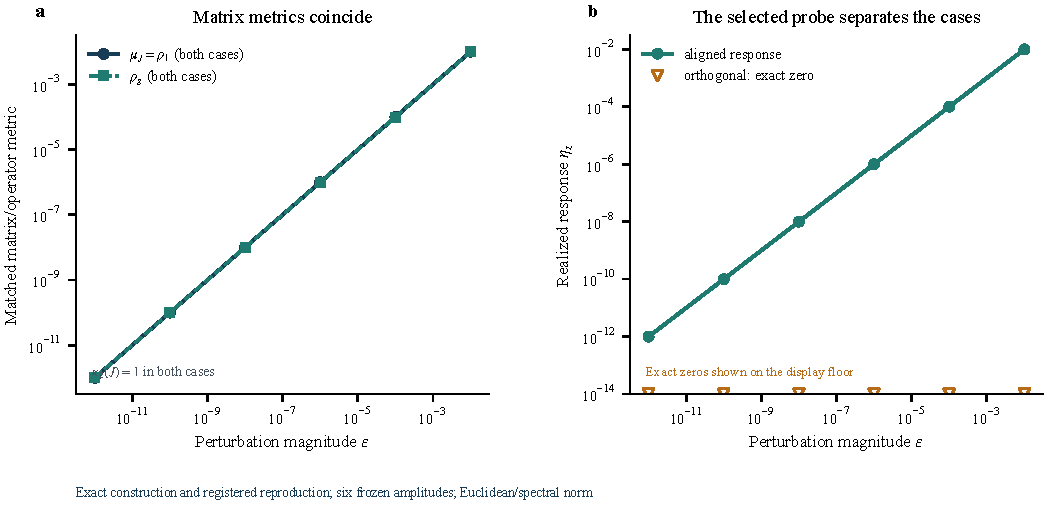
\includegraphics[width=0.92\linewidth,height=0.62\textheight,keepaspectratio]{F3_directional_response.pdf}
\caption{Aligned and orthogonal realized responses under matched matrix and worst-direction quantities for six pre-specified perturbation amplitudes.}
\label{fig:3}
\end{figure}

\begin{linenomath*}
\begin{equation}
\eta_z(A)=\frac{\varepsilon}{1+\varepsilon},
\qquad \eta_z(B)=0.
\label{eq:p2_realized_response}
\end{equation}
\end{linenomath*}

The pre-specified numerical reproduction evaluated six frozen amplitudes from $1\allowbreak\times10^{-12}$ to $1\allowbreak\times10^{-2}$ using an independent high-precision route for the exact construction. Across all six rows, the maximum relative difference between the paired matrix metrics was $0$, the maximum relative error in the nonzero aligned response was $8.721173782511926\allowbreak\times10^{-102}$, and the maximum absolute orthogonal response was $0$. These values reproduce the analytical metric match and the response distinction without changing the construction after observation. The numerical verification validates implementation of this exact example; it does not add an empirical frequency statement. In particular, six amplitudes for one two-dimensional construction are not an operator-family survey, and the zero response in case B follows from exact orthogonality rather than from a general perturbation-screening rule.

\begin{linenomath*}
\begin{equation}
\begin{aligned}
\max \delta_{\mathrm{matched}} &= 0,\\
\max \delta_{\eta_A} &= 8.721173782511926\times10^{-102},\\
\max |\eta_B| &= 0.
\end{aligned}
\label{eq:p2_reproduction_accuracy}
\end{equation}
\end{linenomath*}

The logical content of P2 is an existence result. It shows that scalar matrix amplitude, a condition-number comparison, and even a matched worst-direction finite operator norm are insufficient to reconstruct $\eta_z$ for one selected right-hand side. It does not estimate how often alignment or orthogonality occurs, assign probabilities to response levels, classify either perturbation for practical use, or infer behavior under spatial refinement. The pre-specified reproduction strengthens confidence that the exact construction was evaluated as specified, but it does not enlarge the theorem's domain. Any claim about a family of coupled operators would require a separately designed family, declared sampling rule, and evidence appropriate to that population. Accordingly, P2 is used here only to establish non-determination of a directional response by the matched matrix metrics.

\FloatBarrier
\section{Coordinate-Transformation Verification}
\label{sec:coordinate}

Let the physical unknown and scaled unknown be related by the nonsingular matrix $D_x$, and let residual coordinates be transformed by the nonsingular matrix $D_r$. The frozen convention is $z = D_x \widehat z$ and $\widehat r = D_r^{-1} r$. Substitution into $r = Jz-b$ defines the scaled operator and right-hand side as $\widehat J = D_r^{-1} J D_x$ and $\widehat b = D_r^{-1}b$. A perturbation belongs to the same operator relation and must therefore transform as $\widehat{\Delta J} = D_r^{-1} \Delta J D_x$. These equations define equivalent coordinates only when the unknown, residual, right-hand side, operator, and perturbation are transformed together. Applying a transformation to some objects while independently redefining another object creates a different perturbed problem, even if the same numeric symbol is displayed. Scaling and equilibration literature motivates explicit coordinate declarations but does not supply unique physical choices for $D_x$ and $D_r$ \cite{S05,S06,S07,S08}.

\begin{linenomath*}
\begin{equation}
\begin{aligned}
z&=D_x\widehat z, & \widehat r&=D_r^{-1}r,\\
\widehat J&=D_r^{-1}JD_x, & \widehat b&=D_r^{-1}b,\\
\widehat{\Delta J}&=D_r^{-1}\Delta J D_x.
\end{aligned}
\label{eq:coordinate_transform}
\end{equation}
\end{linenomath*}

Suppose first that the perturbation is declared in physical coordinates as $\Delta J_{\mathrm{phys}} = \varepsilon I$. Its representation in the scaled operator is obtained by the joint transformation, giving $\widehat{\Delta J} = \varepsilon D_r^{-1}D_x$. The transformed perturbation is a scalar identity only when $D_r^{-1}D_x$ is a scalar multiple of the identity, and it retains the same $\varepsilon I$ representation only when $D_x = D_r$. In a mixed-dimensional system, different unknown and residual scales generally make the diagonal entries field dependent. This is a coordinate statement: it identifies the scaled representation of one fixed physical operator. It neither changes that operator nor evaluates the practical consequences of its action. Treating the transformed matrix as if it had to retain the original scalar identity form would replace transformation by redeclaration.

\begin{linenomath*}
\begin{equation}
\Delta J_{\mathrm{phys}}=\varepsilon I,
\qquad \widehat{\Delta J}=\varepsilon D_r^{-1}D_x.
\label{eq:physical_identity_transform}
\end{equation}
\end{linenomath*}

The reverse construction begins with a perturbation declared in scaled coordinates as $\widehat{\Delta J} = \beta I$. Mapping it to physical coordinates gives $\Delta J_{\mathrm{phys}} = \beta D_r D_x^{-1}$, which is generally a field-dependent diagonal operator. Thus a dimensionless identity guard denotes a family of physical perturbations indexed by the declared unknown and residual scales. The mapping does not select those scales; it only states which physical operator corresponds to the scaled identity after the coordinate contract is fixed. Consequently, the label $\beta I$ is incomplete without the operator space, $D_x$, $D_r$, and the direction in which the transformed solution is interpreted. This distinction also prevents a same-numeric identity written in two coordinate systems from being treated as one perturbation without checking the transformation rule.

Figure~\ref{fig:4} distinguishes equivalent coordinate transformation from same-numeric-label redeclaration.

\begin{figure}[htbp]
\centering
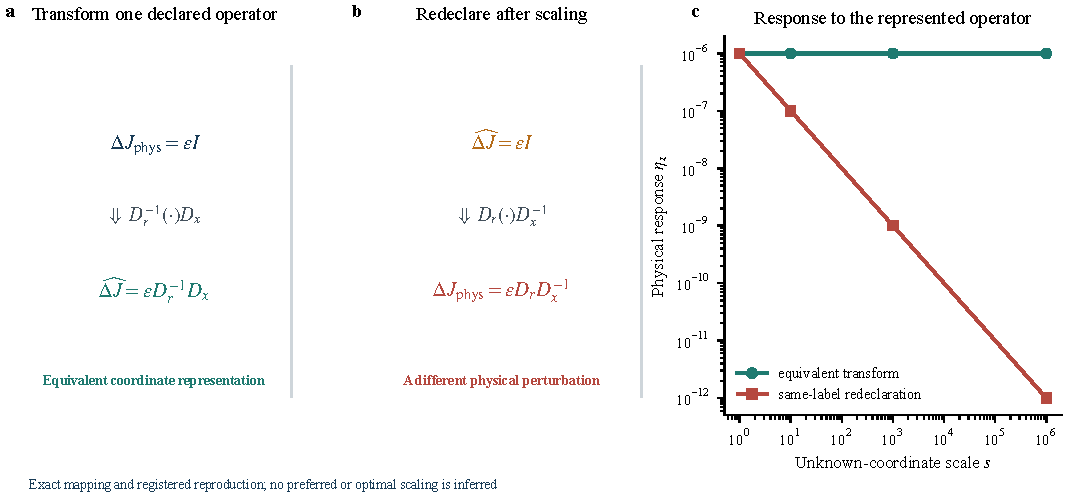
\includegraphics[width=0.90\linewidth,height=0.62\textheight,keepaspectratio]{F4_coordinate_transformation.pdf}
\caption{Equivalent coordinate transformation and same-numeric identity redeclaration under the declared coordinate convention.}
\label{fig:4}
\end{figure}

\begin{linenomath*}
\begin{equation}
\widehat{\Delta J}=\beta I,
\qquad \Delta J_{\mathrm{phys}}=\beta D_rD_x^{-1}.
\label{eq:scaled_identity_mapping}
\end{equation}
\end{linenomath*}

The equivalent-transformation calculation used a two-dimensional construction with pre-specified scale factors $1$, $10$, $1\allowbreak\times10^{3}$, and $1\allowbreak\times10^{6}$. In the equivalent transformed-operator route, the unknown, right-hand side, operator, and perturbation were transformed consistently. The resulting maximum relative difference between physical-equivalent perturbation operators was $7.490674676829096\allowbreak\times10^{-102}$, and the relative spread of the physical response was $0$. These results validate the implemented transformation for the frozen construction and pre-specified scales. They do not establish that arbitrary independently specified guards are invariant; invariance here follows because the transformed descriptions represent the same physical operator and the same physical solution response. The numerical values therefore check the algebraic mapping rather than define a coordinate-independent scalar guard.

\begin{linenomath*}
\begin{equation}
\begin{aligned}
\max \delta_{\mathrm{operator}} &= 7.490674676829096\times10^{-102},\\
\operatorname{spread}(\eta_z)_{\mathrm{transformed}} &= 0.
\end{aligned}
\label{eq:p3_reproduction_accuracy}
\end{equation}
\end{linenomath*}

The second pre-specified lane reapplied the same numeric identity after changing coordinates instead of transforming the original perturbation. With $D_r=I_2$ and $D_x=\operatorname{diag}(1,s)$, that scaled identity maps back to a physical perturbation whose second diagonal entry is $\varepsilon/s$, whereas the original physical identity retains $\varepsilon$ on both diagonal entries. The two physical perturbations coincide at $s=1$ and differ for every pre-specified $s>1$; the pre-specified inequality check was therefore true. The same-numeric-label redeclaration result demonstrates that a shared numeric label does not establish operator equivalence. It does not show that one of the resulting operators should be selected. The observed response change follows from comparing different physical perturbations, not from a failure of coordinate transformation.

\begin{linenomath*}
\begin{equation}
\Delta J_{\mathrm{redeclared}}\neq
\Delta J_{\mathrm{transformed}}\quad\text{for every pre-specified }s>1.
\label{eq:p3_redeclaration_result}
\end{equation}
\end{linenomath*}

P3 establishes a declaration requirement, not a scale-selection method. Neither the algebraic mapping nor the pre-specified verification identifies unique physical scales, an optimal equilibration, field weights, or a coordinate system with preferable solution behavior. Equilibration can alter numerical conditioning, while physical nondimensionalization can encode modeling choices, but those purposes require separate criteria and evidence \cite{S07,S08}. The result here is narrower: a perturbation comparison is meaningful only after the coordinate transformation and operator identity have been fixed. A future analysis may compare alternative scale declarations, but it must treat them as different study designs unless their operators, data, and response coordinates are transformed equivalently. This boundary prevents a coordinate label from being converted into an assessment of perturbation quality.

\FloatBarrier
\section{Uncertainty-Model Validation}
\label{sec:uncertainty}

Let $z$ and $z_g$ denote exact solutions in one declared truth lane, and let $\widetilde z$ and $\widetilde z_g$ be the corresponding computed parent solutions. Direct subtraction produces $\delta_{\mathrm{obs}} = \operatorname{fl}(\widetilde z_g-\widetilde z)$, whereas the exact response is $\delta z=z_g-z$. The computed parents are represented as $\widetilde z=z+e$ and $\widetilde z_g=z_g+e_g$, and the rounded vector subtraction contributes an additional error $q$. These definitions separate the mathematical response from its computed observation. A direct difference can be interpreted only relative to bounds for both parent-solution errors and the subtraction error, all expressed in the same coordinates and norm. IEEE arithmetic and forward-error analysis motivate this separation, but they do not provide an application-specific budget without verified operands and solves \cite{S09,S10,S11}.

\begin{linenomath*}
\begin{equation}
\begin{aligned}
\widetilde z &= z+e, & \widetilde z_g &= z_g+e_g,\\
\delta_{\mathrm{obs}}&=\operatorname{fl}(\widetilde z_g-\widetilde z)
=\delta z+e_g-e+q.
\end{aligned}
\label{eq:computed_difference_model}
\end{equation}
\end{linenomath*}

Proposition P4 assumes valid bounds $\lVert e \rVert\leq U_z$, $\lVert e_g \rVert\leq U_{z_g}$, and $\lVert q \rVert\leq U_{\mathrm{sub}}$ and defines $U_{\mathrm{direct}}=U_z+U_{z_g}+U_{\mathrm{sub}}$. The triangle inequality then gives $\lVert \delta_{\mathrm{obs}}-\delta z \rVert\leq U_{\mathrm{direct}}$, while the forward and reverse triangle inequalities enclose the exact response norm between $\max(0,d_{\mathrm{obs}}-U_{\mathrm{direct}})$ and $d_{\mathrm{obs}}+U_{\mathrm{direct}}$, where $d_{\mathrm{obs}}=\lVert \delta_{\mathrm{obs}} \rVert$. If $d_{\mathrm{obs}}>U_{\mathrm{direct}}$, zero is excluded under that pre-specified error model. The conclusion is conditional: invalid or mismatched parent bounds invalidate the distinguishability statement even if the subtraction itself is evaluated exactly. A small linear residual or backward error alone is insufficient because forward error also depends on problem sensitivity \cite{S03,S11}. P4 therefore supplies no fixed binary64 threshold; it specifies what an uncertainty argument must cover.

\begin{linenomath*}
\begin{equation}
\begin{aligned}
U_{\mathrm{direct}}&=U_z+U_{z_g}+U_{\mathrm{sub}},\\
\lVert\delta_{\mathrm{obs}}-\delta z\rVert&\leq U_{\mathrm{direct}},\\
\max(0,d_{\mathrm{obs}}-U_{\mathrm{direct}})
&\leq\lVert\delta z\rVert\leq d_{\mathrm{obs}}+U_{\mathrm{direct}}.
\end{aligned}
\label{eq:direct_difference_enclosure}
\end{equation}
\end{linenomath*}

\begin{quote}
\textbf{Definition (uncertainty-qualified distinguishability from zero).}
Under a declared truth contract, response route, coordinate system, norm, and route-specific uncertainty model, a computed nonnegative response $d_{\mathrm{obs}}$ with certified absolute uncertainty bound $U$ is \emph{distinguishable from zero} when
\begin{equation}
d_{\mathrm{obs}}-U>0.
\label{eq:distinguishable_definition}
\end{equation}
The statement excludes zero only under the declared uncertainty model. It does not establish a prescribed relative accuracy unless a separate accuracy criterion is declared, and it does not establish physical or engineering significance, guard safety or harm, or nonlinear consequence. The decision is route- and truth-contract-specific; it introduces no free numerical threshold.
\end{quote}


The revised P4 uncertainty model implements this conditional logic through two non-interchangeable truth contracts. The decimal-source reference lane treats the pre-specified decimal operators and right-hand sides as the source problem, while the binary64-operand reference lane treats the exact reconstructed binary64 operands supplied to the solver as a separate real-valued problem. Writing $A_s x_s=b_s$ and $A_b x_b=b_b$ for the source and binary parent problems, respectively, and $\widetilde x$ for either computed parent, each solution is compared with the residual and inverse norm of its own lane. The common subtraction allowance uses the frozen binary64 unit roundoff, a one-operation factor, the absolute parent operands, and an underflow allowance. The source and binary parent envelopes are then combined with the same subtraction term, but each total is compared only with its corresponding response truth. This non-mixing rule is necessary because decimal-to-binary representation and guarded-matrix construction can change the source problem before linear-solve error is assessed. Higher precision supports a reference only when its implementation and operation graph are independently checked \cite{S12,S13}.

Figure~\ref{fig:5} keeps the decimal-source and binary64-operand reference contracts separate.

\begin{figure}[htbp]
\centering
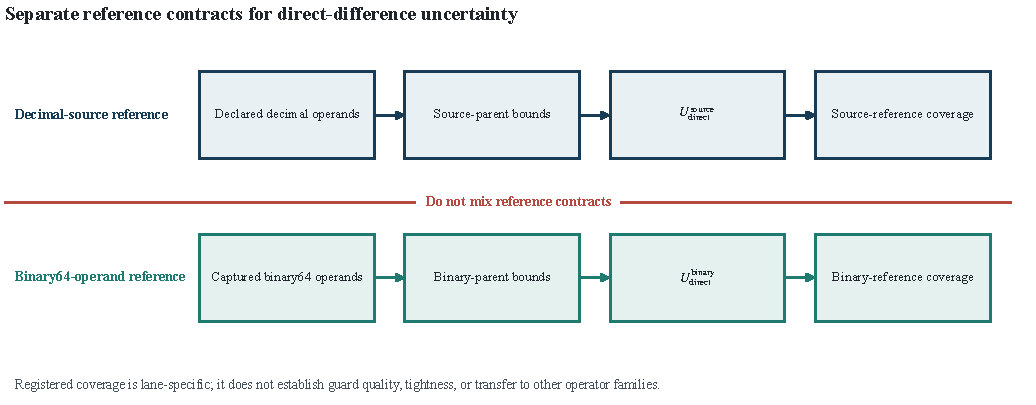
\includegraphics[width=0.90\linewidth,height=0.62\textheight,keepaspectratio]{F5_two_reference_contracts.pdf}
\caption{Separate decimal-source and binary64-operand reference contracts used to construct route-specific error enclosures.}
\label{fig:5}
\end{figure}

\begin{linenomath*}
\begin{equation}
\begin{aligned}
A_s x_s &= b_s, & A_b x_b &= b_b, & u&=2^{-53},\\
\gamma_1&=\frac{u}{1-u},\\
U_{\mathrm{parent},s}&=\lVert A_s^{-1}\rVert_F
\lVert b_s-A_s\widetilde x\rVert_2,\\
U_{\mathrm{parent},b}&=\lVert A_b^{-1}\rVert_F
\lVert b_b-A_b\widetilde x\rVert_2,\\
U_{\mathrm{sub}}&=\gamma_1\lVert|\widetilde z_g|+|\widetilde z|\rVert_2
+\sqrt{n}\,2^{-1075},\\
U_{s}&=U_{\mathrm{parent},s}(z)+U_{\mathrm{parent},s}(z_g)+U_{\mathrm{sub}},\\
U_{b}&=U_{\mathrm{parent},b}(z)+U_{\mathrm{parent},b}(z_g)+U_{\mathrm{sub}}.
\end{aligned}
\label{eq:two_truth_uncertainty_model}
\end{equation}
\end{linenomath*}

Before revision, the pre-specified historical direct envelope was reproduced exactly on the 300-case development family. It covered $287/300$ response differences and recorded three severe undercoverage cases. The frozen revision contract identified a mismatch in the historical truth specification: the historical parent-solve envelopes were formed relative to rounded binary operands, while the reference response was defined by the pre-specified decimal source operators. Under the decimal-source truth contract, the historical envelope therefore omitted a source-representation response component. This attribution motivated separate source and binary lanes; it did not change the historical result or assign the misses to the matrix perturbation itself. Exact reproduction of $287/300$ and three severe cases was required before the revised model was evaluated.

The revised model was first evaluated on the frozen 300-case development set comprising SPD, nonsymmetric, and saddle-point-like decimal families with dimensions $2$, $4$, $8$, and $16$. The source envelope covered $300/300$ decimal-source reference-response errors, and the binary envelope covered $300/300$ binary64-operand reference-response errors. The pre-specified counts of severe undercoverage, parent-component bound failures, subtraction-bound failures, and nonfinite results were all zero. The maximum reference relative residual was $6.15236029869614753170882916397730867400586658\allowbreak\times10^{-105}$, below the pre-specified tolerance of $1\allowbreak\times10^{-70}$. These results validate source and binary error coverage for the development design. They do not evaluate bound tightness and do not extend the error model to operator dimensions outside the pre-specified family.

The disjoint holdout used the same three construction families and dimensions but a frozen independent seed, different condition-exponent grid, and different guard-amplitude grid. Its source envelope covered $300/300$ decimal-source reference-response errors, and its binary envelope covered $300/300$ binary64-operand reference-response errors. Severe undercoverage, component-bound failures, subtraction-bound failures, and nonfinite results again had zero counts, and two complete evaluator runs were exactly repeatable. The development and holdout results therefore provide complete pre-specified coverage on the development and holdout sets in both truth lanes. Because the holdout remains within the pre-specified construction families and dimensions, it tests disjoint pre-specified cases rather than unrestricted matrix systems. No extrapolation to dimensions $196$ or $900$ follows from these results.

Table~\ref{tab:2} summarizes historical reproduction and pre-specified development and holdout coverage.

\begin{table}[htbp]
\centering
\small
\caption{Historical reproduction and development/holdout coverage in the two declared truth lanes.}
\label{tab:2}
\begin{tabularx}{0.98\textwidth}{@{}>{\raggedright\arraybackslash}p{0.24\textwidth}>{\raggedright\arraybackslash}p{0.23\textwidth}>{\raggedright\arraybackslash}p{0.20\textwidth}X@{}}
\toprule
\textbf{Dataset/lane} & \textbf{Coverage} & \textbf{Severe undercoverage} & \textbf{Evidence role} \\
\midrule
historical development & 287/300 (13 uncovered) & 3 & reproduced motivation \\
development source & 300/300 (0 uncovered) & 0 & pre-specified coverage \\
development binary & 300/300 (0 uncovered) & 0 & pre-specified coverage \\
holdout source & 300/300 (0 uncovered) & 0 & pre-specified coverage \\
holdout binary & 300/300 (0 uncovered) & 0 & pre-specified coverage \\
\bottomrule
\end{tabularx}

\end{table}

Figure~\ref{fig:6} reports development and holdout coverage separately from the descriptive tightness diagnostic.

\begin{figure}[htbp]
\centering
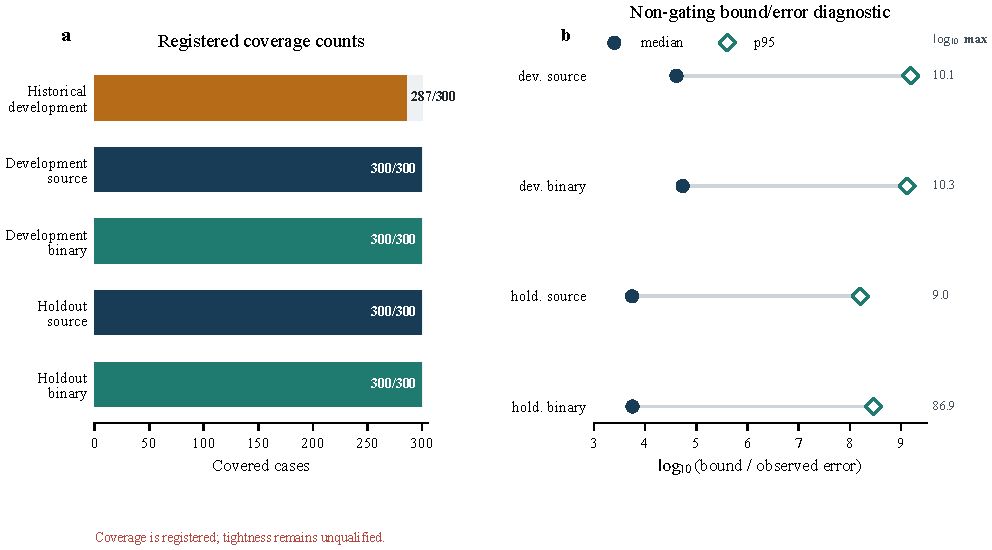
\includegraphics[width=0.92\linewidth,height=0.62\textheight,keepaspectratio]{F6_coverage_and_tightness.pdf}
\caption{Historical, development, and holdout coverage together with the non-gating bound-to-error diagnostic.}
\label{fig:6}
\end{figure}

Coverage and tightness answer different questions. The coverage criteria ask whether every modeled error is enclosed; they do not limit how conservative an enclosure may be. A post-execution descriptive diagnostic reported median bound-to-error ratios of $4.096571\allowbreak\times10^{4}$ and $5.405257\allowbreak\times10^{4}$ for the development source and binary lanes, respectively, and $5.565432\allowbreak\times10^{3}$ and $5.666318\allowbreak\times10^{3}$ for the holdout source and binary lanes. These ratios show that many bounds exceed their corresponding observed errors by substantial factors, as expected from a direction-independent inverse-Frobenius envelope applied to directional response errors. No tightness criterion was pre-specified, so the diagnostic cannot validate estimator efficiency or class sharpness. The result supports decimal-source and binary64-operand reference-error coverage; the present limitation is that the absence of a tightness qualification remains in force.

Figure~\ref{fig:7} records the source-contract attribution of the three historical severe-undercoverage cases without assigning a guard defect.

\begin{figure}[htbp]
\centering
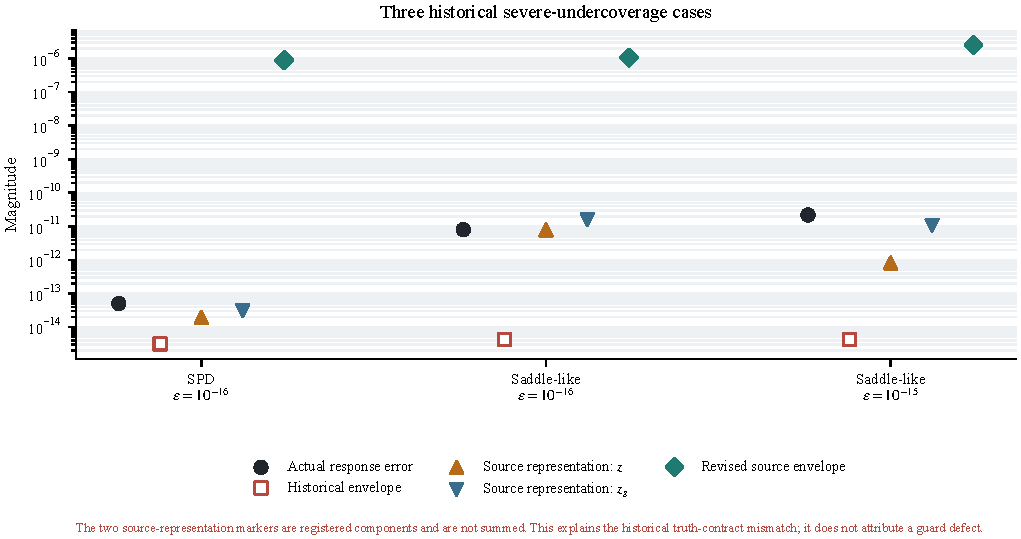
\includegraphics[width=0.92\linewidth,height=0.62\textheight,keepaspectratio]{F7_historical_undercoverage_attribution.pdf}
\caption{Source-representation attribution for the three historical severe-undercoverage cases.}
\label{fig:7}
\end{figure}

The exact P1 identity also permits a response solve, $(J+\Delta J)\delta z=-\Delta J z$, that avoids direct subtraction of two full computed solutions. In a selected pre-specified small-perturbation subset, this route had a reported win rate of $1$ relative to direct subtraction and a median error ratio of $6.835288346086798\allowbreak\times10^{-10}$. This observation is diagnostic motivation only. A computed response solve inherits error from the parent solution used to form $\Delta J z$, arithmetic used to construct that product, and the subsequent solve. It is therefore not an authoritative truth route without its own forward-error enclosure or independent higher-precision comparison \cite{S03,S11,S13}. Avoiding one subtraction changes the error pathway; it does not remove the need to validate that pathway.

The validated scope of the revised P4 uncertainty model is confined to the pre-specified SPD, nonsymmetric, and saddle-point-like decimal families, dimensions $2$, $4$, $8$, and $16$, and their disjoint holdout, for a total of 600 evaluated cases. The construction supplies evidence across several operator forms, condition grids, and perturbation amplitudes, but it does not establish coverage for unrestricted operator populations or for larger frozen mixed-field tangents. In particular, no case-matched decimal-source reference verification was pre-specified for dimensions $196$ or $900$, and no mesh-independent coverage law was tested. The framework can be applied to another operator only after its solved space, coordinates, norms, perturbation, right-hand side, parent error bounds, subtraction bound, precision, and truth route are declared and validated. This boundary keeps pre-specified coverage separate from future generalization. Coverage is jointly a property of the sampled operator family, the declared truth route, the precision used to construct the operands, and the particular error envelope; changing any of these objects defines a new validation problem rather than a continuation of the pre-specified one. The presence of SPD, nonsymmetric, and saddle-point-like families broadens the frozen test design, but finite samples from those families cannot establish behavior for every member of the corresponding mathematical classes. Likewise, disjoint holdout construction reduces reuse of the development grid but does not supply an external population model. Future extension to larger mixed-field systems would therefore require case-matched source and binary operands, an independent reference route, pre-specified forward-error components, and a new holdout whose design is fixed before response results are inspected. These requirements are methodological consequences of the coverage claim's scope, not evidence that the current envelopes will fail or succeed outside it.

The pre-specified validation scope was limited to decimal-source and binary64-operand reference-error coverage. All 300 development systems and all 300 holdout systems were covered in each truth lane, with no severe undercoverage. The study did not qualify the tightness of the resulting envelopes.

\FloatBarrier


\section{Applications to Two Coupled Finite-Element Linearizations}
\label{sec:applications}

\subsection{Frozen operators and route definitions}

The application stage uses two independently frozen transformed free-system snapshots. M8 is a $196\times196$ nonsymmetric tangent with 5442 stored nonzeros; M16 is a $900\times900$ nonsymmetric tangent with 28259 stored nonzeros. Each snapshot fixes the IEEE binary64 matrices $J$ and $J_g$, the common right-hand side $b$, the free-degree-of-freedom ordering, the unknown and residual scales, and the Euclidean comparison norm before either response route is evaluated. The perturbation is reconstructed as $\Delta J=J_g-J$ and is diagonal in both snapshots. Figure~\ref{fig:8} shows the two sparsity patterns and their independently qualified response intervals.

The truth object for each application is the real-valued system represented exactly by the captured binary64 operands. Integer-ratio reconstruction, signed-zero checks, and the identity $J_g=J+\Delta J$ establish that operand contract before high-precision evaluation. Parent systems and the response equation are then solved independently at 120 and 180 decimal digits. The direct-difference route evaluates $\operatorname{fl}(\widetilde z_g-\widetilde z)$ and includes both parent-solution and subtraction components. The response-equation route evaluates $(J+\Delta J)\delta z=-\Delta Jz$ and uses its own parent, forcing-construction, and response-solve components. Each route is compared only with its matching uncertainty enclosure.

\begin{figure}[htbp]
\centering
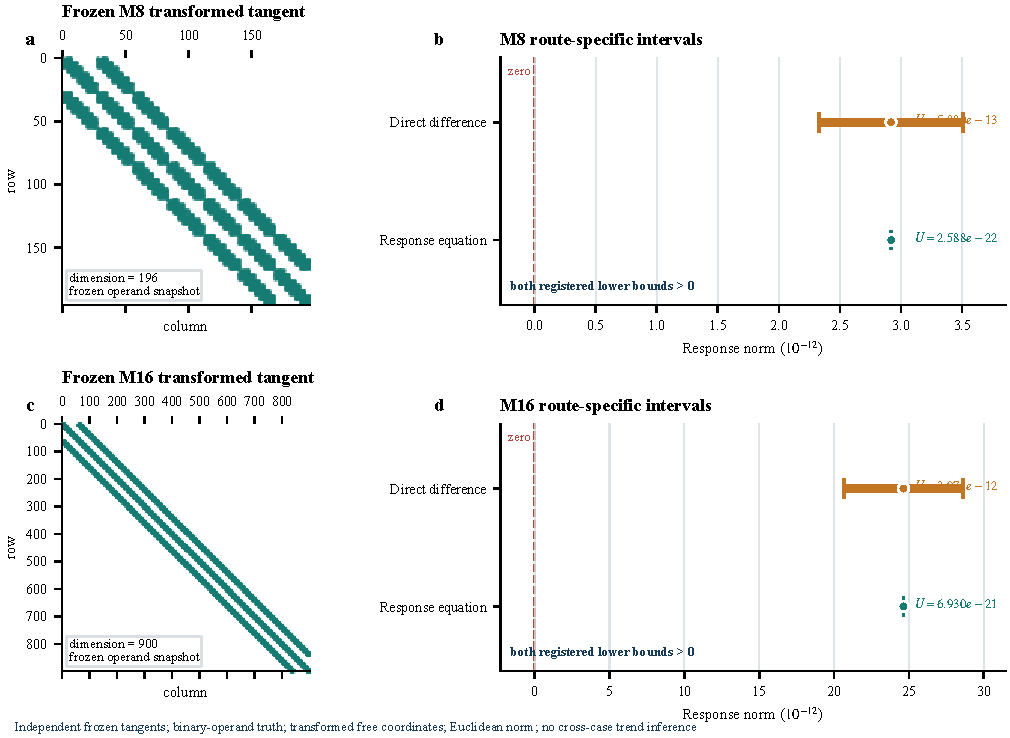
\includegraphics[width=0.98\linewidth,height=0.72\textheight,keepaspectratio]{F8_two_operator_route_qualification.pdf}
\caption{Route-specific response qualification for two independently frozen coupled finite-element tangents. Panels show the M8 and M16 sparsity patterns and the direct-difference and response-equation intervals; dashed references denote zero.}
\label{fig:8}
\end{figure}

\subsection{M8 application}

For M8, the maximum normalized difference between the 120- and 180-digit references was $8.805709238088443\times10^{-121}$, the maximum reference relative residual was $2.550975633144060\times10^{-124}$, and the response-identity difference was $9.184908547614584\times10^{-123}$. Independent-process repetitions reproduced the reference and binary-route artifacts exactly.

The direct-difference route produced $d_{\mathrm{obs}}=2.918501453675816\times10^{-12}$ and $U=5.880137782404462\times10^{-13}$, giving the positive lower bound $2.330487675435369\times10^{-12}$ and a relative-error upper bound of approximately $0.2523136$. The response-equation route produced $d_{\mathrm{obs}}=2.920014225448921\times10^{-12}$ and $U=2.588299567178917\times10^{-22}$, again giving a positive lower bound. Both M8 responses are therefore distinguishable from zero under their respective route-specific enclosures.

\subsection{M16 application}

For M16, the maximum 120/180-digit normalized difference was
\[
3.970070132750439\times10^{-121}.
\]
The maximum reference relative residual was $4.144081636789256\allowbreak\times10^{-124}$, and the response-identity difference was $3.042263371127549\allowbreak\times10^{-122}$. A separate process reproduced both precision references, route artifacts, and decisions exactly, with no mutation of the operand snapshot.

The direct-difference route produced $d_{\mathrm{obs}}=2.463376440770722\allowbreak\times10^{-11}$ and $U=3.970799910942942\allowbreak\times10^{-12}$, giving the lower bound $2.066296449676427\allowbreak\times10^{-11}$ and a relative-error upper bound of approximately $0.1921699$. The response-equation route produced $d_{\mathrm{obs}}=2.463671846097062\allowbreak\times10^{-11}$ and $U=6.930482617167356\allowbreak\times10^{-21}$, giving the positive lower bound $2.463671845404014\allowbreak\times10^{-11}$. Both M16 responses are distinguishable from zero under their own enclosures. Exact decimal strings and uncertainty components are retained in Supplementary Tables~S4--S6.

\subsection{Replication and offline cost}

Table~\ref{tab:3} summarizes the four case-route results without combining them into an estimator score. Completing the same declaration, reference, uncertainty, and zero-exclusion sequence for both M8 and M16 demonstrates replication of the assessment procedure on two frozen coupled finite-element linearizations. The cases were not selected or controlled as a mesh, dimension, or conditioning sequence, so their values do not define a cross-case trend or a universal ranking of the arithmetic routes.

\begin{table}[htbp]
\centering
\scriptsize
\caption{Route-specific response qualification for the two frozen finite-element tangents. Displayed values are rounded; Supplementary Table~S4 retains the exact decimal strings.}
\label{tab:3}

\resizebox{\linewidth}{!}{%
\begin{tabular}{@{}llrrrrrl@{}}
\toprule
\textbf{Case} & \textbf{Dimension} & \textbf{Route} & \textbf{Observed response} & \textbf{Uncertainty bound} & \textbf{Lower bound} & \textbf{Rel.-error upper bound} & \textbf{Decision} \\
\midrule
M8 & 196 & Direct difference & $2.918501\times 10^{-12}$ & $5.880138\times 10^{-13}$ & $2.330488\times 10^{-12}$ & $2.523136\times 10^{-1}$ & Distinguishable \\
M8 & 196 & Response equation & $2.920014\times 10^{-12}$ & $2.588300\times 10^{-22}$ & $2.920014\times 10^{-12}$ & $8.863996\times 10^{-11}$ & Distinguishable \\
M16 & 900 & Direct difference & $2.463376\times 10^{-11}$ & $3.970800\times 10^{-12}$ & $2.066296\times 10^{-11}$ & $1.921699\times 10^{-1}$ & Distinguishable \\
M16 & 900 & Response equation & $2.463672\times 10^{-11}$ & $6.930483\times 10^{-21}$ & $2.463672\times 10^{-11}$ & $2.813071\times 10^{-10}$ & Distinguishable \\
\bottomrule
\end{tabular}%
}

\end{table}

The complete M8 offline calculation, including both precision levels and an independent repeat, required 467.5920785~s and 115154944 bytes of peak memory in the recorded environment. M16 required 37512.1609418~s and 1452195840 bytes. These two observations are computational provenance rather than a complexity fit. They show that the present high-precision route is an offline qualification oracle. Sparse updates, inverse-norm estimators, verified sparse solvers, and precision-aware refinement offer relevant directions for a scalable estimator \cite{S26,S27,S28,S31}, but any replacement route would require an independent accuracy and coverage study.

\FloatBarrier
\section{Discussion}

\subsection{Why matrix magnitude is insufficient}

The analysis separates questions that are often compressed into one statement about a small matrix term. The ratio $\mu_J$ measures amplitude in declared coordinates, $\rho_1$ and $\rho_g$ measure inverse-mediated worst-direction amplification, and $\eta_z$ measures the response of one selected right-hand side. Proposition P2 shows that even matched values of $\mu_J$, $\rho_1$, $\rho_g$, and $\kappa(J)$ do not determine $\eta_z$. Directional information enters through $\Delta Jz$ and its propagation by the perturbed inverse. Condition-number comparisons therefore remain useful bounds, but not directional mechanism classifiers \cite{S01,S02,S03}.

\subsection{Why coordinate declaration matters}

The matrix representation of a perturbation changes with unknown and residual coordinates. Under $z=D_x\widehat z$ and $\widehat r=D_r^{-1}r$, a physical identity perturbation becomes $\varepsilon D_r^{-1}D_x$, while a dimensionless identity maps back as $\beta D_rD_x^{-1}$. The coordinate verification confirms equivalent responses only when the operator, data, and perturbation are transformed together. Reusing the same numeric identity after changing coordinates declares a different physical operator. The procedure consequently requires a solved-space and coordinate contract before any matrix ratio or response comparison is interpreted; it does not prescribe a preferred nondimensionalization or equilibration \cite{S05,S06,S07,S08,S29}.

\subsection{Why distinguishability differs from accuracy and physics}

The test $d_{\mathrm{obs}}-U>0$ answers one numerical question: whether zero is excluded under the declared truth object, arithmetic route, and uncertainty model. Coverage asks whether the model enclosed known reference errors over a specified family, whereas relative accuracy requires an additional ratio criterion. Physical significance requires a problem-dependent response scale or consequence. These are separate statements. The complete development and holdout coverage supports the two declared truth lanes within the evaluated families; the finite-element applications support route-specific zero exclusion for their captured operands.

\subsection{Why arithmetic routes require separate uncertainty models}

Direct subtraction and the response equation implement the same exact response identity through different floating-point operation graphs. Direct subtraction inherits the errors of two parent solves and the subtraction itself. The response equation inherits error from the parent used to construct $\Delta Jz$, the forcing construction, and the response solve. A tighter interval for one route in M8 or M16 is therefore a case-specific consequence of these decompositions. It cannot establish a universal route ordering. This separation is also why small parent residuals alone do not qualify a computed difference: a backward-error statement does not supply every forward-error component required by the response route \cite{S03,S09,S10,S11}.

\subsection{Replication across two finite-element linearizations}

The same ten-stage procedure was completed independently for the 196- and 900-dimensional tangent snapshots. Both applications fixed the operand and coordinate contracts before route evaluation, reconstructed binary64 operands exactly, used independent precision ladders, and qualified both response routes through their own enclosures. This closes the methodological question of whether the complete procedure can be repeated on more than one coupled finite-element linearization. Because the two snapshots do not form a designed sequence or statistical sample, the replication does not estimate a mesh law, dimension dependence, or frequency over an operator population.

\subsection{Offline oracle versus scalable estimator}

Independent dense high-precision solves provide a clear offline truth route but do not scale as an online production diagnostic. The recorded M8 and M16 costs make this limitation visible without defining a performance law. Scalable alternatives may combine sparse factor updates, inverse-norm estimation, verified sparse solves, or precision-aware refinement \cite{S12,S26,S27,S28,S31}. Translating the present method to such an estimator requires more than replacing the arithmetic kernel: the estimator must preserve the solved-space and coordinate declarations, expose route-specific uncertainty, and be validated for coverage against an independent reference.

\subsection{Limitations}

The method assesses a tangent-only matrix perturbation at a declared linearization. It does not convert that perturbation into a residual-consistent stabilization and does not infer mixed-method stability, conservation, boundedness, physical importance, or a subsequent nonlinear trajectory. Synthetic uncertainty coverage is confined to the pre-specified operator families and dimensions, while the application evidence is confined to two frozen binary64 snapshots. Table~\ref{tab:4} summarizes these interpretation boundaries once, rather than attaching the full list to every result.

\begin{table}[htbp]
\centering\small
\caption{Interpretation boundary by claim domain. Supplementary Table~S7 retains the complete claim--evidence matrix.}
\label{tab:4}

\begin{tabularx}{\linewidth}{@{}>{\raggedright\arraybackslash}p{0.18\linewidth}>{\raggedright\arraybackslash}X>{\raggedright\arraybackslash}X@{}}
\toprule
\textbf{Domain} & \textbf{Established} & \textbf{Not established} \\
\midrule
Theory & Finite response identity, directional non-determination, and coordinate mapping under declared assumptions. & Prevalence, optimal scaling, or a universal guard rule. \\
Synthetic evidence & Pre-specified reproduction and coverage on the frozen development and disjoint holdout designs. & Unrestricted-system coverage or estimator tightness. \\
Frozen tangents & Route-specific qualification completed separately for M8 and M16. & Mesh law, dimension trend, or population-level generality. \\
Route comparison & Each route has its own uncertainty components and a case-specific decision. & Universal route ranking or superiority. \\
Interpretation & Numerical distinguishability under declared contracts. & Guard safety or harm, nonlinear consequence, finite-element stability, or engineering qualification. \\
Cost & Recorded offline cost and resource provenance for each frozen case. & Online estimator feasibility, complexity fit, or production scaling. \\
\bottomrule
\end{tabularx}

\end{table}

Within these limits, the contribution is a computational assessment procedure rather than a perturbation-selection algorithm. It makes the represented operator explicit, separates matrix, operator, and directional quantities, and requires uncertainty matched to the arithmetic route before a computed response is classified.

\FloatBarrier

\section{Conclusions}

This study developed a scale-explicit and uncertainty-qualified procedure for assessing a tangent-only matrix perturbation in a coupled finite-element linearization. The procedure declares the solved space and coordinates, separates matrix amplitude from inverse-mediated and directional response measures, and qualifies the selected response through a route-specific error enclosure.

An exact finite identity establishes the response relation, while a matched two-dimensional construction proves that matrix and worst-direction quantities do not determine one realized response. Coordinate-transformation verification shows why identity perturbations require explicit operator-space declarations. Development and disjoint holdout families then validate the two-contract uncertainty model within their specified operator classes and dimensions.

The complete procedure was independently applied to frozen 196- and 900-dimensional coupled finite-element tangents. Direct-difference and response-equation intervals excluded zero in both applications under their own uncertainty models. The two cases establish replication of the method, while their route values remain application specific.

The present high-precision implementation is an offline qualification oracle, and the two frozen applications do not establish population-level generality or nonlinear and engineering consequences. Future work should address scalable route-specific uncertainty estimators for large sparse nonlinear finite-element linearizations rather than extending the current offline oracle by brute force.

\section*{Data availability}
The non-confidential frozen operands, synthetic validation records, exact-value tables, claim--evidence matrix, and provenance files supporting this study are archived in Zenodo at \href{https://doi.org/10.5281/zenodo.21833851}{https://doi.org/10.5281/zenodo.21833851} \cite{liang2026artifact}. The archive excludes Abaqus executables, user-element source, solver state histories, and engineering project data.

\section*{Code availability}
The scripts for the analytical constructions, uncertainty-model validation, and the two offline finite-element linearization applications are available at \href{https://github.com/yqma7980/scale-explicit-matrix-perturbation-observability}{https://github.com/yqma7980/scale-explicit-matrix-perturbation-observability} and are preserved with the cited Zenodo release. Code is licensed under the MIT License; data and documentation are licensed under CC BY 4.0.

\section*{Reproducibility statement}
The reported calculations use immutable operand snapshots, explicit coordinate and truth contracts, two independent precision levels, independent-process repeatability checks, and exact output records. The Supplementary Information retains full numerical precision, uncertainty components, and execution provenance.

\section*{CRediT authorship contribution statement}
\textbf{Bing Liang:} Conceptualization, Methodology, Formal analysis, Writing -- original draft, Writing -- review and editing, Supervision. \textbf{Yangqi Ma:} Methodology, Software, Validation, Formal analysis, Investigation, Data curation, Visualization, Writing -- original draft, Writing -- review and editing. \textbf{Weiji Sun:} Conceptualization, Methodology, Resources, Supervision, Project administration, Funding acquisition, Writing -- review and editing. \textbf{Shi He:} Methodology, Validation, Writing -- review and editing.

\section*{Funding}
This work was supported by the National Natural Science Foundation of China (General Program, Grant No. 52474038, awarded to Weiji Sun).

\section*{Declaration of competing interest}
The authors declare that they have no known competing financial interests or personal relationships that could have appeared to influence the work reported in this paper.

\section*{Declaration of generative AI and AI-assisted technologies in the writing process}
During preparation of this work, the authors used Codex (OpenAI) to assist with language revision, document organization, and consistency checks. The authors reviewed and edited all affected content and take full responsibility for the content of the publication.

\bibliographystyle{elsarticle-num}
\bibliography{Paper2_CMAME_references_v0.6}

\end{document}
